\documentclass{article}

\usepackage[margin=0.5in]{geometry}
\usepackage{amsmath, amssymb, changepage, tikz-cd, mathtools}

\newcommand{\n}{\leavevmode \newline}
\newcommand{\nn}{\leavevmode \newline \newline}
\newcommand{\R}{\mathbb{R}}
\newcommand{\C}{\mathbb{C}}
\newcommand{\st}{\text{ s.t. }}
\newcommand{\sti}{\textit{ s.t. }}
\newcommand{\Hom}{\text{Hom}}

\begin{document}

\title{Linear Algebra Notes (DRAFT)}
\author{Piyush Patil}
\date{June 21, 2017}
\maketitle

TODO: recast symmetric matrices as linear maps equivalent in both a basis and the corresponding dual basis

\section{Vector Spaces}

The central object of study in linear algebra is the vector space. Vector spaces are inherently algebraic objects, and are thus best motivated algebraically. They're special versions of the more general algebraic structure: modules. To review, let's briefly go over the fundamental underlying algebraic structures.

\begin{enumerate}

    \item \textit{Groups}: A group is one of the most general yet powerful algebraic structures studied in algebra. It equips to a set a quite sparse structure that nonetheless remains powerful enough to encompass and generalize an enormous number of domains, settings, and spaces of interest in all branches of mathematics. It imbues a set of elements with a single binary operation - simply a way to "combine" elements of the set, in such a way as to remain within the set - which is forced to satisfy a few axiomatic conditions to ensure the "niceness" of the resulting structure when we manipulate it. These axioms are: \textit{associativity}, so that the order in which we combine elements shouldn't matter, \textit{identity}, which guarantees the existence of an element in the set that's invariant under the operation and therefore intuitively serves as a kind of unique grounding element for the whole set, and \textit{invertibility}, which allows us to undo our operation when we please. Associativity exists so that our operation acquiesces to our intuitive notion of how a "combiner" of elements should behave, since in most natural settings if we're combining different things, the order in which we combine them shouldn't matter, but rather merely that the ingredients were combined at all (though the sequence in which they were combined might be relevant, as in a recipe). Identity grounds the set, and moreover is necessary to define invertibility, and invertibility is a very important axiom since it's what allows us to actually do "algebra", in the traditional sense of the word, within our group; it allows us to put forth, transform, study, solve, and otherwise manipulate equations and relations between elements and operations between them.
    \item \textit{Rings}: Rings extend groups by throwing in an additional operation. To motivate them, we begin with a commutative group, meaning not only does the order in which we combine elements not matter, but nor does the sequence in which we combine elements (hence, the nature of this binary operation is that it cares only about the characteristics of the elements being combined, and not about the order, sequence, or any other kind of "metadata" of the elements; in this sense, it's completely faithful to the elements it's combining themselves, with no added subterfuge in its action). This binary operation is often called \textit{addition}, owing to its being motivated as a generalization of addition as defined over the integers. In this same vein of motivation, we extend this additive commutative group with the intention of introducing a way to also combine integers in a more complex way, one that's almost built from or on top of addition - \textit{multiplication}. Thus, rings also have another binary operation, called multiplication, which is required only to be associative and have an identity (for the same reason as with group operations). Finally, we require a distributivity law to connect the two operations.
    \item \textit{Field}: A ring in which multiplication is invertible (except possibly at the additive identity, which is a generalized case of "division by zero").
    \item \textit{Modules}: Modules are motivated by the canonical examples of a vector space: $ \R^n $, or the set of $ n $-tuples of real numbers. Immediately from the definition, there are a few natural things we can do with these $ n $-tuples: we can add them quite easily, with a simply, natural generalization of how we add real numbers (i.e. component-wise), and we can scale them, with a similar generalization of how we multiply real numbers (i.e. again, component-wise). Modules generalize this idea; a module over a ring is a commutative group of elements (this allows us to add elements in a well-behaved way) equipped with a left multiplication operator between elements of the group and the underlying ring. The underlying ring here acts like a set of well-behaved scalars, which can interact with each other in pleasing ways but which can also the main objects of our study - elements of the overarching additive group - by "acting" on them through a left multiplication. To cement this intuition, we force this left multiplication to conform to a few axioms of its own: it should be associative, so that consecutively left multiplying by two rings elements should be the same as multiplying the ring elements first and then acting on the group element, and distributive over both ring addition and the group addition. These two axioms are what tie the two algebraic structures together, both as groups and as a ring and group, in a tight-knit, simple way which generalizes and combines both algebraic structures. Finally, we require that the multiplicative ring identity act on group elements exactly as we'd expect: by doing nothing.
    \begin{enumerate}
        \item Notice right off the bat that all commutative groups are automatically modules over the ring of integers, if we simply have integers act on group elements in the most canonical, natural way we can extend integer multiplication: as iterated addition, so that for any integer $ n $ and group element $ G $, $ n \cdot g = g + \cdots + g (n \text{times}) $, where $ + $ is the group operation, and negative integers do the same thing but on $ g $'s inverse instead.
        \item Also notice that any commutative ring (a ring where multiplication is also commutative) is a module over itself, if we just have the ring multiplication double as the action of the "underlying" ring on group elements (in this case really ring elements, of course).
    \end{enumerate}
\end{enumerate}

A vector space is simply a module in which the underlying ring is actually a field. Vector spaces are often called linear spaces, especially in functional analytic contexts, because of their inherently "linear" structure. Consider what it is we can do in a vector space. We have a central group of elements, called vectors, that we can add together in a basic way that depends only on the vectors themselves, and not their order or any other external attribute. We can scale these vectors up and down by acting on them with scalars, thought of here simply as numbers that obey a "linear" structure of their own (after all, we can add and multiply them in precisely the same generalized senses as we can add vectors). Further, the way in which we scale vectors and add vectors need to play nice with each other, again in a very linear way - the two must distribute. This, combined with the existence of scalar and additive identities, imbues an inherently linear structure on the space - combining scalars then scaling a vector is the same as consecutively scaling twice, combining two vectors and then scaling is the same as scaling each then combining, we add vectors in a way that generalizes the addition of real numbers, which is in turn motivated by a simple translation or shift of the real line (obviously a very "linear" way of transforming the real line; all we're doing here is moving it over).
\nn
These characteristics enforce a strict linear structure on the elements of a vector space, and though our intuition for this idea was informal, vague, and non-rigorous, this idea will become increasingly clear and precise the more we study vector spaces. In particular, we're going to motivate and demonstrate that vector spaces, which were themselves motivated by $ n $-tuples of real numbers, are actually just copies of their underlying scalar field glued together, the same way $ \R^n $ is $ n $ copies of $ \R $ glued together. Once proven, this theorem is simple but incredibly far-reaching and powerful, showing us that all vector spaces merely do is take the inherently linear, simple, symmetric structure of a field of scalars, and constructing a space by merely slapping copies of this field orthogonal to each other; it's exactly the same idea as $ n $-dimensional Euclidean space.
\nn
To go forth doing this, we'll need to talk about the idea of a direct sum (which formalizes the "gluing" process above). The notion is simple. The Cartesian product is a set operation (meaning an operation over sets) which is how we "multiply" two sets; what it does it take two sets, place them perpendicular to each other, and look at pairwise combinations of elements of the two sets. As far as operations over sets go, it's quite dull, seeing as the two sets being combined don't really interact in any meaningful way, but it does capture our intuitive notion of "gluing" together orthogonal sets, turning two 1-dimensional objects into a single 2-dimensional object formed by multiplying them. A direct sum is an operation over groups which takes the Cartesian product, and gives the resulting the set the simplest, most dull and natural possible structure - elements of the direct sum are added with component-wise addition of elements of the two underlying groups. We can extend this to apply to modules too, if the modules are over the same ring: just have ring elements act on elements of the direct sum in a component-wise way. The direct sum is denoted with the infix operator $ \oplus $, so $ G \oplus H $ is the direct sum of groups $ G, H $. Now, the theorem we alluded to above is framed as showing that any vector space is just a direct sum of copies of its underlying field.
\nn
Before formally stating this theorem, let's use direct sums to define some useful intermediate concepts. When we motivated direct sums, we referenced the idea that the resulting structure was of a higher dimension than the ones from which it was built. At its most general, the term "dimension" can taken to mean an independent, orthogonal direction that contains new information not contained in other dimensions (otherwise it'd be degenerate and wouldn't really be a "new" direction in our space), closely related to the statistical idea of a degree of freedom. Taking the direct sum of $ n $ modules should, as per this intuition, yield an  $ n $-dimensional space. Let's try to define the dimension of a vector space in a way that captures these ideas.
\nn
Recall that given vectors of a module, we can scale them and add them together. Taking $ n $ vectors, scaling each one, and then adding the results is called a linear combination; intuitively, it's just a weighted sum. If we have a set of vectors for which no linear combination (that is, no matter what weights we choose) degenerates to zero (here referring to the additive vector identity), then we say the vectors are linearly independent. This is a very useful definition. If we have $ n $ vectors, then their linear combination is the most general way of combining them within their containing vector space; varying this linear combination over different possible weights generates a set of new vectors, each of which is "built" from our original set. If, even by varying a linear combination over all possible weights, we still can't hit zero, then this new set of generated vectors makes full, complete, non-redundant use of each of the $ n $ vectors we started with, in the following sense: every vector in the generated set is built from the original $ n $ vectors and hence can be specified with the corresponding $ n $ weights, and if the vectors are linearly independent, then the specification of $ n $ weights not only contains sufficient information to identify that vector, but is a "maximal entropy", information theoretically optimal such specification - removing even a single piece of information would destroy the entire representation and disallow us from identifying vectors in the generated set. This can be seen more clearly by considering the converse - in a linearly dependent set of vectors, it follows directly that at least one of the vectors is a linear combination of the others, and so the generators of the generating set actually contain something that was already in the generating set to begin with. Surely this is redundant; why include something as a fundamental generator necessary to represent elements in a generated set when that object can be expressed in terms of the other generators anyways? We call this generated set the spanning set of the $ n $ vectors, i.e. the set of all linear combinations of the vectors, taken over all permutations of $ n $ scalars. Geometrically, expressing a vector as a linear combination amounts to starting at the origin of a space and explaining how to reach the vector by traversing pre-determined directions in the space, generalizing, for instance, the cardinal directions on a map.
\nn
Sometimes it turns out that the spanning set of a set of vectors is actually the entire containing vector space, so every vector is a linear combination of our generators. If, in addition, the generating vectors are linearly independent, we call the set of these vectors a basis. Intuitively, vectors in a basis fully generate the entire vector space, and so every vector in the space can be represented by telling us how to reach it by following the elements of the basis; since the basis is linearly independent, this representation is both complete and non-redundant. It's easy enough to prove that this linear independence condition is equivalent to having the linear combination representation of vectors be unique. Here we can now see a generalized sense of how we use "coordinates" in $ n $-dimensional Euclidean space, since after all we just defined a way to uniquely and completely specify vectors in the space, now regarded as points, with tuples of scalars (namely, the weights in the unique linear combination). This is also how we'll now define the term "dimension" as promised above. It follows from the above ideas we discussed about bases that any two bases of a vector space have the same size. Intuitively, this is because if you have a basis, then adding in another vector is redundant since that vector can already be expressed as a linear combination of the basis, and so the result is not a basis; if two different bases have different numbers of vectors, the larger one would hence be forced to contain something that's redundant and couldn't be a basis. The dimension of a vector space is defined as the number of vectors in its basis (yes, every vector space has a basis).
\nn
Note here that again, the fact that all vector spaces are generated by linear combinations of some basis (most often more than one basis, of course) is more evidence of the inherent linear structure of vector spaces. Also note that this definition of dimension really only makes sense when bases are finite, but infinite dimensional vector spaces do in fact exist (such as the vector space of polynomials).
\nn
An extremely ubiquitous idea in mathematics is that of a structure-preserving mapping. From isomorphisms to homeomorphisms to diffeomorphisms and so on, it's extremely common (and in fact one of the central lines of inquiry in category theory) to consider different instances of some mathematical object, structure, or space and see what properties they have in common. Morphisms in particular are bijective maps between two mathematical objects which completely preserve all the relevant structure of the two objects. This means that if we have two mathematical objects in some context and the corresponding morphism between them, the two objects are actually one and the same, merely represented differently. Isomorphic groups share every relevant group property, homeomorphic topological spaces share all relevant topological properties, and so on; these morphisms are merely ways of telling us how different parts of one structure correspond to parts of the other structure, in such a way that both parts play the exact same role relative to every other part in the encompassing local and global contexts. When it comes to vector spaces, the relevant structure we wish to preserve is, of course, the inherent linear structure, and hence the relevant structure-preserving maps to consider are linear maps between vector spaces, more commonly called linear transformations.
\nn
Linear transformations are defined precisely as maps which are linear, in the sense that they decompose over addition (so a linear map $ T $ satisfies $ T(v + w) = T(v) + T(w) $ for vectors $ v, w $) and factor through scaling (so a linear map $ T $ satisfies $ T(c \cdot v) = c \cdot T(v) $ for scalar $ c $ and vector $ v $). This is a standard definition of linearity, extended from the quintessential examples of linear objects - the familiar lines in the Euclidean plane through the origin, which have the unmistakable, essential linear property of mapping changes in input to directly proportional changes in output. Thus, linear transformations generalize real-valued linear functions of the form $ f(x) = m x $ for real $ m $. It happens by design that this definition of a linear transformation also preserves all the relevant structure necessary to identify vector spaces with each other, owing again to the linear structure of vector spaces. In fact, a bijective (meaning both the map and its inverse are one-to-one and hence the map acts as a perfect "lookup table") linear transformation is precisely an isomorphism between vector spaces, and hence if there exists a bijective linear transformation between two vector spaces, the spaces are really the same space, merely expressed in different representations and symbols. By applying ideas related to the basis, the dimension of a vector space, and linear transformations on that vector space, it's not hard to prove the central theorem we alluded to above, which we can now formally state as follows: every $ n $-dimensional vector space over a field $ F $ is isomorphic to the $ n^\text{th} $ direct sum of $ F $ (defined as the direct sum of $ F $ with itself $ n $ times). The core idea behind the proof is that once we pick a relevant basis, we can uniquely and completely express any vector in the vector space with an $ n $-tuple of scalars from $ F $, known as its coordinates with respect to that basis, and because of the linear nature of a vector space, addition and scaling reduce to component-wise operations anyways, and hence what we're left with is a simple linear structure applied to $ n $-tuples in $ F $, i.e. $ F $ glued to itself $ n $ times.
\nn
One caveat to note here: though every $ n $-dimensional vector space (over some fixed field of scalars) is isomorphic to the same direct sum, to reduce every vector space to this direct sum would still throw away a lot of the relevant structure of the vector space that goes beyond its linear structure. For example, we could identify the space of polynomials of degree at most $ n $ with $ \R^n $, but to do so would disallow us from studying properties of polynomials embedded in the vector space. Moreover, the isomorphism in question feels a bit arbitrary, since there are many possible isomorphisms and each depends on your choice of basis, which of course doesn't and shouldn't matter at all since they just express the same space in different ways. Yes, we could recast a vector space as a set of $ n $-tuples of scalars with some linear structure, with each vector corresponding to some $ n $-tuple, but to do so would require us to make the completely arbitrary decision of which $ n $ scalars to use. This alludes to a wider problem in linear algebra, and in particular to the way it's taught and the misconceptions that result. Vectors, at their core, are certainly not just arrays of $ n $ numbers; rather, their defining quality is that they are elements of an enclosing vector space, subject to certain relationships and structure. Simply because we can represent them as arrays of $ n $ scalars doesn't mean there's anything particularly special or illuminating about this representation; after all, there are often infinitely many bases of a vector space, each providing a new, unique representation of the same vector. Throughout the remainder of this entry, we'll be drawing a major distinction between ideas and results which are basis-free (also referred to as coordinate-free), meaning they hold true independent of what basis we pick and are thus more canonical and essential than their counterparts, and those that require some specific basis to be true. The fact that vector spaces are isomorphic to direct sums of their underlying field relies on a specific, arbitrary choice of basis to construct this isomorphism, and hence is not basis-free and intuitively much less ideal and pure than we'd expect from an isomorphism. We'll later take a look at which vector spaces are truly isomorphic, in a basis-free, canonical sense.
\nn
Having introduced linear transformations, let's now take a look at one of their most well known, if not misconstrued, associates - matrices. The first thing to notice here is that going off our intuition for what a basis is, namely a way of minimally representing the whole space through a set of generators, it's not unreasonable to expect that many properties and manipulations of vector spaces can be reduced to the special case of what happens at the basis vectors. When it comes to linear transformations, this is exactly the case - because linear transformations decompose over vector addition and pass right through scalar multiplication, this means that linear transformations act on linear combinations of some vectors in a way that's fully determined by those vectors. Since every vector in a vector space is a unique linear combination of basis vectors (with respect to some arbitrary basis), the the linear transformation is completely determined by it's behavior at the basis vectors. Symbolically,
	$$ \forall v: \exists \textit{ scalars } c_i \textit{ (for $ 1 \leq i \leq n $)} \sti v = c_1 v_1 + \cdots + c_n v_n $$
and therefore
	$$ T(v) = T(c_1 v_1 + \cdots + c_n v_n) = c_1 T(v_1) + \cdots + c_n T(v_n) $$
within some vector space, where $ T $ is a linear transformation and the $ v_i $ form a basis. Now suppose $ T $ is a linear transformation from a vector space $ V $ to a vector space $ W $; we know it's determined by it's action on some basis for $ V $, say $ \{ v_i, 1 \leq i \leq n \} $; namely, $ T $'s behavior decomposes naturally into the vectors $ T(v_i) $ in $ W $. We can further express each $ T(v_i) $ as a linear combination of basis vectors of $ W $, for some basis, say $ \{ w_j, 1 \leq j \leq m \} $. The matrix representation of $ T $ is defined simply as an array of length $ n $ whose entries are vertical arrays of coordinates of the $ T(v_i) $. Put more explicitly, we define the rectangular array of scalars
	$$ \begin{aligned}
		A &= \begin{bmatrix} T(v_1) & \cdots & T(v_n) \end{bmatrix} \textit{where } T(v_i) = a_{1, i} w_1 + \cdots + a_{m, i} w_m \textit { for scalars } a_{j, i} \textit{ over } 1 \leq i \leq n \textit { and } 1 \leq j \leq m \\
		&= \begin{bmatrix}V
			a_{1, 1} & \cdots & a_{1, n} \\
	  		\vdots & \ddots & \vdots \\
		    a_{1, m} & \cdots & a_{m, n}
	    \end{bmatrix}
	\end{aligned} $$
to be the matrix induced by $ T $. The definition of matrix multiplication is precisely so that this matrix representation of a linear transformation faithfully reflects the identity
	$$ T(v) = T(c_1 v_1 + \cdots + c_n v_n) = c_1 T(v_1) + \cdots + c_n T(v_n) = \begin{bmatrix} T(v_1) & \cdots & T(v_n) \end{bmatrix} \cdot \begin{bmatrix} c_1 & \cdots & c_n \end{bmatrix}^\intercal = A \begin{bmatrix} v \end{bmatrix} $$
where $ \begin{bmatrix} c_1 & \cdots & c_n \end{bmatrix}^\intercal $ is the coordinate representation of $ v $ (the transpose is just to signify that this is a column vector), denoted $ \begin{bmatrix} v \end{bmatrix} $, relative to the basis $ \{ v_1, \cdots, v_n \} $. Extending this definition to matrix-matrix multiplication allows us to naturally represent the composition of linear transformations as matrix multiplication.
\nn
So, yes a matrix is a rectangular array of scalars, but which scalars depends on the (totally arbitrary) choice of bases in the domain and co-domain. This is where the definition of similar matrices comes from - recall that matrices $A $ and $ B $ are similar if there exists an invertible matrix $ P $ such that $ A = P B P^{-1} $; this condition essentially uses $ P $ as a change of basis matrix whose columns are basis vectors, and hence states that A is simply a version of $ B $ converted to a different basis over the same vector space; in other words, $ A $ and $ B $ represent the same linear transformation, just with respect to different bases. A matrix is just a convenient numerical (in terms of the underlying field, of course, and not necessarily real numbers, though the reals (as well as the complex numbers) do tend to be the most common choice of scalar field) representation of a linear transformation relative to a particular basis. Nonetheless, in accordance with our distinction between basis-free and basis-dependent definitions and theorems, the most prominent essence of the idea behind a matrix is that it is a representation of a linear transformation between vector spaces that allows us to work with the algebra of linear transforms using natural, numerical form of generalized multiplication and addition (incidentally this is also very helpful in applied settings from a computational perspective), and decidedly not that it's a just a rectangular array of numbers we can manipulate according to strange rules.
\nn
From this perspective, the various diverse applications and properties of matrices make much more sense and take on their appropriate positions in a deeper logical context. For example, invertible matrices correspond to linear transformations with linear inverses, and hence linear transformations that are isomorphisms, which incidentally is why they have full rank and span the whole space (if they didn't they certainly couldn't be isomorphisms). It's why matrices can be used to represent a system of linear equations: since a vector space is equivalent to gluing a scalar field to itself many times over, taking $ n $ equations over those scalars and necessitating that they be satisfied simultaneously is equivalent to simply defining a generalized linear equation - using an $ n $-dimensional linear transformation instead of $ n $ 1-dimensional linear functions - over the $ n^\text{th} $ direct sum of that scalar field. It's why row operations are valid: since matrices are defined in terms of the action of the associated linear transformation on basis vectors, and because given a basis, interchanging two basis vectors or scaling a basis vector doesn't change the basis, it's permissible to scale and swap rows (or columns, since swapping columns only changes the order in which coordinates are specified, which also has no effect on the underlying basis) without altering the intrinsic nature of the matrix relative to the overarching vector space in which it's defined. It's why matrix multiplication is associative but not commutative: function composition satisfies this exact condition. The list continues - every elementary property of matrices one might encounter is merely some simple, often intuitive or even obvious, small combination of properties of linear transformations and vector spaces, and indeed this is the perspective one should adapt in buttressing the lens through which one works with and manipulates matrices. As we'll see below, this perspective will also allow us to give meaning to concepts such as the determinant, the trace, transposes, the adjoint, etc.
\nn
A slight digression on the behavior of linear transformations:
\n
\begin{adjustwidth}{1cm}{1cm}

	Though linear transformations are basis-independent, there are certain bases under which their action on the space reduces to a particularly simplistic and aesthetically pleasing form, a form which also turns out to be very useful in deducing exactly what a linear transform does to a vector space. This form will be stated in terms of the kernel of a linear transformation (the \textit{kernel} is defined simply as the set of stuff a linear transformation kills by mapping to zero), a particularly important subspace of a vector space when it comes to linear transformations, defined to be the set of elements that a transform maps to zero. Given any linear transformation $ T $ between vector spaces, we can find bases $ \{ v_i, 1 \leq i \leq n \} $ and $ \{ w_j, 1 \leq j \leq m \} $ for the domain and co-domain, respectively, such that there exists some index $ k $ so that
		$$ \forall i \leq k: T(v_i) = w_i $$
		$$ \forall i > k: T(v_i) = 0 $$
	Before unpacking what this theorem actually tells us, notice again that this statement, which we'll soon show to be a penetrating insight into the structure of linear transformations and a hidden connection to group theory, is a statement on which matrices are diagonalizable and which aren't; we'll connect this statement to well-known facts about matrix diagonizability when we encounter eigenspaces. The above statement is actually fairly easy to prove once we understand what it's really saying. The idea is to pick a basis for the kernel of $ T $, and then extend that basis to a full basis for the whole vector space (call it $ V $). We can perform this extension by simply choosing vectors that are consecutively linearly independent until the number of vectors hits the dimension of $ V $; the key insight is that when it comes to these new vectors we've thrown in, $ T $ must be injective, precisely because by design none of them can be in the kernel of $ T $, which means no linear combination of them can be mapped to zero. Thus, the images of these extra vectors are linearly independent, and form a basis for the co-domain of $ T $ (call it $ W $). Once we extend these images to a full basis the same way we did for $ V $, the statement follows.
	\nn
	The crux of the argument was to recognize that finding the "index boundary" $ k $ for which $ T $ completely preserved basis elements only required us to look at the kernel of $ T $, since it's only within that subspace which $ T $ kills (i.e. maps to zero) that we need to worry about $ T $ mapping linearly independent vectors to linearly dependent vectors. This exposes an interesting symmetry between the structure of $ V $ and the structure of $ W $, when viewed as connected by $ T $ - one part of $ V $ get completely destroyed by $ T $ and the rest gets pristinely preserved. More precisely, this means that we can express $ V $ as the direct sum of $ T $'s kernel and some other subspace (call it $ X $) of $ V $; the action of $ T $, then, is to annihilate its kernel and send $ X $ to a perfectly isomorphic copy of itself within $ W $. Moreover, a corollary of this theorem is the famous rank-nullity theorem:
		$$ \dim(V) = \dim(\text{ker}(T)) + \dim(\text{im}(T)) $$
	Finally, those familiar with some group theory might recognize this fact as reminiscent of the first isomorphism theorem. Indeed, this statement can be reframed in the exact same way. Intuitively, given that $ V = $ direct sum of $ \text{ker}(T) $ and $ X $, and that $ \text{im}(T) $ is isomorphic to $ X $, it's intuitive that if we "quotient" $ V $ by $ \text{ker}(T) $ to undo the direct sum, the result would be identical to the action of $ T $, so that $ T $ is an isomorphism between the "quotient vector space" (yes, this isn't rigorously defined but bear with me) $ V / \text{ker}(T) $ and $ \text{im}(T) $ as embedded in $ W $.

\end{adjustwidth}

\section{Traces and Determinants}

As promised, let's use our newfound perspective (at least in contrast to the one meagerly provided by the primary mode of education in elementary linear algebra) to motivate, define, extent, and analyze two very powerful concepts surrounding linear transformations: the determinant and trace. In so doing, we'll explore some rich algebraic theory as well as the connections between the trace and determinant to the more advanced theory of linear maps and spaces.
\nn
First, a brief roadmap. The trace and determinant are often defined in a way that seems highly dependent on the positional entries of a matrix, in a strange, nebulous way. To give a basis-free definition of these concepts and link it to the more obscure, computational definitions, we'll need to introduce entirely new, more advanced ways of exploring the relationship between a linear transformation and its induced matrix representation. This means we'll be shifting our perspective slightly, moving from vector spaces as our primary object of study to linear transformations; we'll be looking at the set of all linear transformations between two vector spaces, and using tools from group, ring, and module theory to study the imposed algebraic structure on this set and its relationship to matrices. We'll start by studying the trace. To do so, we'll first talk about tensor products, which will allow us to "multiply" vector spaces, and then talk about the dual space of a vector space. Tensor products will be instrumental in looking at the relationship a vector space has with its dual. Finally, We'll use both these concepts in conjunction to get an algebraic feel for the ring of linear transformations between two vector spaces, and use this intuition to cast the trace of a matrix as a composition of two natural, important maps on this ring. As for the determinant, we'll first introduce wedge products, leaning on our intuition for tensor products, of which the former are an extension, and connect the product to our instinctive feel for ideas of area, volume, and beyond in linear contexts. We'll then use wedge products to define the determinant as a spatial or (hyper-)volumetric way of discussing the action of a linear transformation on its domain.
\nn
Onwards to tensor products.

\subsection{Tensor Products}

There's a reason direct sums are called sums - intuitively, as an operation on spaces, they really only "glue" the spaces together in a way that has an unmistakable additive feel to it; after all, there's no sense of scaling involved at all. More rigorously, the dimension of the direct sum is the sum of the dimensions of the operand vector spaces, which confirms the idea that a direct sum really only slaps two vector spaces together in a way that doesn't scale the structure of one by that of the other as we'd expect from a product, as opposed to a sum. Tensor products are a way to define a true product on a vector space, in a way that both satisfies the intuition we seek and maintains a linear structure on the resulting space. If we have two vector space and corresponding bases, we'd expect the product of the spaces to have a basis made up of pairwise products of the elements of the bases of the vector spaces. Direct sums certainly don't accomplish this, since although they use a Cartesian product to achieve a sort of multiplication of basis elements, their algebraic structure is component-wise, defeating the entire purpose of this product structure. Instead, what we seek is to form a new basis of elements which are true (pairwise) products of the two original bases, in a way that behaves exactly as we'd expect from a product.
\nn
Say we have two vector spaces, $ V $ and $ W $, over the same field and with respective bases $ \{ v_i, 1 \leq i \leq n \} $ and $ \{ w_j, 1 \leq j \leq m \} $. The direct sum looks at pairs of basis elements $ (v_i, w_j) $ and imposes a component-wise algebraic structure on it. We can define the tensor product by doing the same thing, but imposing a product structure instead. We'll take pairs of basis elements $ v_i $ and $ w_j $ and denote their tensor product with $ v_i \otimes w_j $ (a quick word on notation - we could have just struck with using ordered pairs, but since we're moving beyond component-wise operations it's less confusing to use an infix operator that, symbolically, looks like and reminds us of multiplication, which after all is the motivating idea we're attempting to generalize here). The tensor product of $ V $ and $ W $, then, is the vector space generated by these algebraic, symbolic elements $ \{ v_i \otimes w_j, 1 \leq i \leq n \text{ and } 1 \leq j \leq m \} $. Let's now impose this product structure on our basis of tensor products. For $ v_i \otimes w_j $ to behave as we'd expect from a product of elements, there are a few axioms we'll require it to satisfy:

\begin{enumerate}
	\item Left distributivity: For any $ v_1, v_2 \in V $ and $ w \in W $: $ (v_1 + v_2) \otimes w = v_1 \otimes w + v_2 \otimes w $
	\item Right distributivity: For any $ v \in V $ and $ w_1, w_2 \in W $: $ v \otimes (w_1 + w_2) = v \otimes w_1 + v \otimes w_2 $
	\item Scalar associativity: For any scalar $ c $, $ v \in V $, and $ w \in W $: $ (c v) \otimes w = v \otimes (c w) $
\end{enumerate}
\n
This definition is bulky but intuitive; more commonly, the tensor product of two vector spaces can be more concisely, cleanly be defined as follows:
\n
\begin{adjustwidth}{1cm}{1cm}
    Given vector spaces $ V $ and $ W $, the pair $ (X, \rho) $, where $ X $ is a vector space and $ \rho: V \times W \rightarrow X $ is a mapping, is said to be the tensor product of $ V $ and $ W $ if the following holds:
        $$ \forall \textit{ bases } \beta_1 \textit{ of } V, \beta_2 \textit{ of } W: \rho \left( \beta_1 \times \beta_2 \right) := \{ \rho(b_1, b_2), b_1 \in \beta_1, b_2 \in \beta_2 \} \textit{ is a basis for } X $$
\end{adjustwidth}
\n
Thus, the tensor product gives us a way of multiplying vectors between two vector spaces; in terms of coordinates, if we have
    $$ v = \begin{bmatrix} c_i \end{bmatrix}_{1 \leq i \leq n}^\intercal \in V \textit{ and } w = \begin{bmatrix} d_j \end{bmatrix}_{1 \leq j \leq m}^\intercal \in W \textit{ for }c_i, d_j \in F $$
where $ F $ is the underlying field, then their product is
    $$ v \otimes w = \begin{bmatrix} c_i \cdot d_j \end{bmatrix}_{1 \leq i \leq n, 1 \leq j \leq m}^\intercal \in V \otimes W $$
Notice that the tensor product isn't commutative. Nonetheless, taken with the above axioms the set of symbols $ \{ v_i \otimes w_j \} $ really does behave like we'd expect from a product of the basis elements, at least with respect to the addition operators defined on each vector space. Moreover, this new basis is linearly independent, which satisfies the motivating deficit we found with using direct sums as a product: $ \dim(V \otimes W) = \dim(V) \cdot \dim(W) $. In this almost hacky, literal sense, the basis of the tensor product is as close to the "product" of the bases of $ V $ and $ W $ as we can get.

\subsubsection{Tensor Algebras}

Let's recap what we've done so far with tensor products, and what it means in the special case of the tensor product of a vector space with itself. The tensor product, then, provides us with a bilinear mapping between vectors in our space, which behaves much as we'd expect multiplication to behave. Recall that in our axiomatic definition of a vector space, we defined an underlying field of scalars and a central commutative group of vectors that can be scaled by these scalars. It made sense to require the scalars compose a field, since our intuitive notion of scaling of magnitudes requires associativity (how we group consecutive scalings shouldn't matter), commutativity (the order in which we scale shouldn't matter), both addition and multiplication (we should be able to additively scale in a linear way, and should be able to multiply scalars so as to enable us to consecutively scale), and invertibility under each (we should be able to undo a scaling operation, of course). However, when considering vectors as independent objects that are themselves scaled, there's no need to sacrifice this much generality by imposing this many axioms. Thus, though we defined a notion of addition between vectors, and a way of scaling them by scalars, we ommitted an actual multiplicative operation between vectors. Indeed, throughout mathematics, both pure and applied, many notions of vector multiplication exist, from the dot product to the cross product. When we take a vector space and equip it with a bilinear multiplication operator, we get what's referred to as an \textit{algebra over a field}. More formally,
\n
\begin{adjustwidth}{1cm}{1cm}
    An \textbf{algebra $ A $ over a field $ F $} is a set of elements $ A $ which is a vector space under addition and scalar multiplication over $ F $, and is further equipped with a binary operator $ \cdot: A \times A \rightarrow A $ such that
    \begin{enumerate}
        \item Right distributivity: $ \forall v, w, x \in A: (v + w) \cdot x = v \cdot x + w \cdot x $
        \item Left distributivity: $ \forall v, w, x \in A: v \cdot (w + x) = v \cdot w + v \cdot x $
        \item Compatibility with scalars: $ \forall v, w \in A, c, d \in F: (c v) \cdot (d w) = (c d) (v \cdot w) $
    \end{enumerate}
\end{adjustwidth}
\n
For example, the complex numbers form a two-dimensional algebra over a field, as do the quaternions and octonions. Notice that the multiplication is required to satisfy no axioms other than bilinearity; it may or may not be associative (in which case $ A $ is an \textit{associative algebra})or commutative (in which case $ A $ is a \textit{commutative algebra}). Algebras with multiplicative identities are called, as with rings, \textit{unital}. Though the tensor product doesn't quite meet our expectations of a product operator, seeing as it doesn't map vectors into the same space, it does form a well-behaved product operator if we first use it to turn our vector space $ V $ into an algebra.
\nn
Before concluding the section on tensor products, we'll cover one final result that hammers home the elegance of tensor products and the role they occupy as cornerstones of mechanisms for combining vector spaces. Specifically, tensor products satisfy a \textit{universal property}. This simply means that when it comes to combining elements from two vector spaces, even in the most general way possible, for all relevant purposes with respect to preserving linearity between linear spaces, we can do no better than considering elements of the tensor product of the two vector spaces, rather than individual elements themselves. In other words, if we have a vector from one vector space and a vector from another, we lost nothing, expressivity-wise, by just considering the tensor product of the two vectors. This idea can be framed formally as follows.
\n
\begin{adjustwidth}{1cm}{1cm}
    For vector spaces $ V $ and $ W $, let $ \phi: V \times W \rightarrow V \otimes W $ be the "tensoring" mapping, i.e. the mapping $ \phi(v, w) = v \otimes W $ for $ v \in V, w \in W $. Then for any vector space $ X $ and bilinear mapping $ f: V \times W \rightarrow X $, we have that $ f $ factors through $ \phi $, meaning there exists a unique $ \widetilde{f}: V \otimes W \rightarrow X $ such that $ f = \widetilde{f} \circ \phi $. In the language of category theory, we have
        $$ 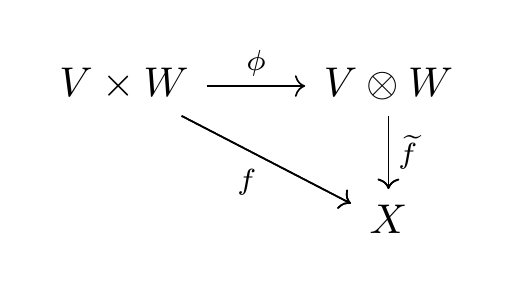
\begin{tikzpicture}[baseline = (a).base]
            \node[scale = 1.5] (a) at (0, 0){
                \begin{tikzcd}
                    V \times W \arrow[rd] \arrow[r, "\phi"] \arrow[rd, "f", swap]
                    & V \otimes W \arrow[d] \arrow[d, "\widetilde{f}"] \\
                    & X
                \end{tikzcd}};
        \end{tikzpicture} $$
\end{adjustwidth}
\nn
Let's now take a look at dual spaces.

\subsection{Dual Spaces}

The definition of a dual space seems strange and counter-intuitive at first, but we'll soon explain where it comes from, and why it's called the "dual". The dual space of a vector space $ V $ is denoted $ V^* $, and is defined as the vector space of linear maps from $ V $ to its underlying field, under the operations of pointwise scalar multiplication and pointwise addition (this just means that for linear maps $ f: V \rightarrow F $ and $ g: V \rightarrow F $ (where $ F $ is the underlying field of $ V $), $ f + g $ is the function given by $ (f + g)(v) = f(v) + g(v) $ for $ v \in V $, and for $ c \in F $, $ c \cdot f $ is the function given by $ (c \cdot f)(v) = c \cdot f(v)) $. Calling this a "dual" space seems to indicate that in some sense $ V^* $ is the other "half" of some larger universe that complements $ V $, akin to a partner in a binary union. This idea is indeed supported by the following fact: the dual of the dual space is isomorphic to the original vector space. In other words, taking the dual of a vector space is an operation that inverts itself, and hence $ V $ and $ V^* $ really are the only two vector spaces dual to each other. Of course, it's easy to point out that of course $ V $ and $ V^* $ are isomorphic; they have the same dimension, and every vector space with the same dimension is isomorphic. However, in this case, we have a very natural, canonical, basis-independent isomorphism that hints towards a truly deeper link between the two spaces. This isomorphism has a natural and pleasing structure: consider $ V^* $, the space of maps which send a linear function between $ V $ and $ F $ to a scalar in $ F $. We can associate any vector $ v \in V $ with an element of $ V^* $ by taking the point evaluation functional at $ v $, defined as the function
	$$ \phi_v: V^* \rightarrow F \sti \forall f \in V^* \textit{ (so $ f: V \rightarrow F $ is a function from $ V $ to $ F $) }: \phi_v(f) = f(v) $$
In other words, the element $ v $ is "grounded" in $ V^* $ by mapping functions on $ V $ to their value at v. This is a completely basis-independent, elegant isomorphism between the spaces. Further, this structure reveals other relationships between $ V $ and $ V^* $ that tie the two spaces inextricably together, in a way that's aesthetically harmonious with the theory of matrices and vectors developed thus far. To see this, recall that a linear transformation can be completely described by its behavior at basis elements. So, once we've chosen some arbitrary basis for our vector space $ V $, not only can we describe the elements of $ V $ with unique lists of $ \dim(V) $ numbers (remember, this is precisely why vector spaces are isomorphic to iterated direct sums of their underlying field), but we can actually do the exact same thing for linear transformations from $ V $ to the underlying field as well (by specifying the images of the linear transform at the basis elements).
\nn
This insight, that grounding a basis for $ V $ allows us to talk about both elements of $ V $ and linear functionals (this is the name we give to linear maps from a space to their underlying field) of $ V $ with $ \dim(V) $ coordinates, reveals a simplistic yet elegant symmetry between the elements of $ V $ and linear functionals on $ V $, and hence between $ V $ and $ V^* $. Consider the following idea: fix a basis $ \{ b_1, \cdots, b_n \} $ for $ V $ and let $ f $ be a linear functional on $ V $; now consider the following row vector (a matrix with a single row, just as column vectors are matrices with a single column)
	$$ \begin{bmatrix} f(b_1) & \cdots & f(b_n) \end{bmatrix} $$
This is exactly the "coordinate description" of $ f $ that we alluded to above, in the same way that column vectors are coordinate descriptions of vectors of $ V $; further, it follows from the way we defined matrix multiplication (and no, this is not a coincidence) that for any vector $ v $ with coordinates $ v_1, \cdots, v_n $, that
	$$ \begin{bmatrix}
		f(b_1) & \cdots & f(b_n)
	\end{bmatrix} \begin{bmatrix}
		v_1 \\
		\vdots \\
		v_n
	\end{bmatrix} = f(b_1) + \cdots + v_n f(b_n) = f(v_1 b_1 + \cdots + v_n b_n) = f(v) $$
What we've shown here is that just as vectors of $ V $ can be represented as column vectors of scalars, the row vectors of scalars on the other hand represent the linear functionals of $ V $. Herein lies the essence of the powerful symmetry between $ V $ and $ V^* $ we've been referencing: linear functionals can be pictured as points in $ n $-dimensional space (here $ n = \dim(V) = \dim(V^*) $) just the same as vectors of $ V $ can be, and conversely vectors of $ V $ can be viewed as linear functionals over $ V $, if we view their coordinates as their "values" at the basis elements; to flit in between these two symmetric, complementary perspectives, we lean on the geometric intuition that $ V $ and $ V^* $ are "perpendicular" rotations of each other. $ V $ and $ V^* $ have the same dimension and are hence isomorphic, and moreover based on the above ideas we can think of $ V^* $ as the result of taking the entire space $ V $ and flipping it by ninety degrees (representing an orthogonal rotation), taking some fixed basis vector as the axis, and further we can go back from $ V^* $ to $ V $ by flipping about this "basis vector axis" ninety degrees the other direction.
\nn
Given this intuition, it shouldn't surprise us that for any basis $ \{ b_1, \cdots, b_n \} $ of $ V $, we can find a dual basis in $ V^* $. Intuitively, we'd expect this dual basis to be the linear functionals corresponding to the row vector representations of $ b_1, \cdots, b_n $, and this is exactly correct. Formally, the following define a basis for $ V^* $
	$$ \textit{ for } 1 \leq i \leq n: \textit{ define } b_i^*: V \rightarrow F \textit{ by } b_i^*(b_j) = \begin{cases}
		1, &\textit{ if } i = j \\
		0, &\textit{ otherwise }
	\end{cases} $$
where again we denote the underlying field of $ V $ as $ F $. Put more simply, $ b_i^* $ is the functional which maps vectors to their $ i^\text{th} $ coordinate with respect to the coordinate representation induced by $ \{ b_1, \cdots, b_n \} $. These functionals precisely correspond with the row vector rotations of the $ b_i $, as can be seen easily by considering the coordinate representations of the $ b_i $ over themselves as a basis and the action of right multiplying with row vectors of the form
	$$ \begin{bmatrix} 0 & \cdots & 0 & 1 & 0 & \cdots & 0 \end{bmatrix} $$
We always knew that $ V $ and $ V^* $ had to be isomorphic, but now we can explicitly nail down exactly what that isomorphism is - simply the one induced by extending the mapping of each $ b_i $ in $ V $ to $ b_i^* $ in $ V^* $. This isomorphism moreover codifies our intuition that $ V^* $ is the result of taking $ V $ and "rotating by ninety degrees", since this is precisely the idea that motivated the isomorphism. Of course, keep in mind that this isomorphism, though geometrically intuitive, is not canonical, as it depends on our choice of basis.

\subsection{The Trace}

We are now in a position to begin exploring the trace. To really understand what the trace is doing, we first need to build a stronger, more rigorous, algebraic intuition for what exactly matrices are relative to their corresponding linear transformations, not just as a convenient numerical representation but in the larger context of the ring of linear transformations between vector spaces. This perspective will further elucidate why matrices are rectangular arrays of rows and columns of scalars, and why this symbolic representation is ideal for linking with a linear transformation in a way that respects the inherent structure of the transform.
\n
\begin{adjustwidth}{1cm}{1cm}

	Let's say we have vector spaces $ V $ and $ W $ (over the same field $ F $), with dimensions $ n $ and $ m $ respectively. Then, as we know, linear maps from $ V $ to $ W $ can be represented as an $ n $ by $ m $ array of scalars. We've already looked at the ring of linear transformations between $ V $ and $ W $, so let's now try to build an algebraic structure of $ n $ by $ m $ scalar arrays, so that we can then show that these two algebraic structures are in fact the same, connected in a fundamental, definitional way. The trivial algebraic way to do this is to use $ F^{nm} $ as this structure, but of course this is neither illuminating nor useful. Instead, we'll use tensor products to build this structure. The reason tensor products are amenable to building this structure is subtly related to the symbolic structure of a matrix - to build an $ n $ by $ m $ matrix, what we're doing is taking length $ n $ row vectors and length $ m $ column vectors and taking some kind of product over them, that extends one vector in the direction of the other, to obtain the $ n $ by $ m $ array. This intuitive idea of taking an $ n $-row vector and extending it $ m $ times perpendicularly (or equivalently taking an $ m $-column vector and extending it $ n $ times) is formalized with the tensor product. We simply take the space of $ n $-row vectors, which as we saw above is the interpretation we gave to the dual space of $ V $, and look at its tensor product with the space of $ m $-column vectors, which is simply $ W $.
	\nn
	To cement the conceptual ideas above, the claim we're making here is that $ V^* \otimes W $, the tensor product $ V $'s dual space with $ W $, is canonically, naturally isomorphic to the ring of linear maps from $ V $ to $ W $ (which, as a relic from ring theory, is denoted $ \Hom(V, W) $, short for "homomorphism ring", but this isn't important). To construct this isomorphism, we need to figure out how to interpret elements of $ V^* \otimes W $ as linear maps. Well, let's say $ \{ b_1^*, \cdots, b_n^* \} $ and $ \{ c_1, \cdots, c_m \} $ are bases for $ V^* $ and $ W $, respectively, so that an element $ M $ of $ V^* \otimes W $ looks like
		$$ M = \sum_{i = 1}^n \sum_{j = 1}^m a_{i, j} \cdot (b_i^* \otimes c_j) \textit{ for scalars } a_{i, j} $$
	In case it wasn't clear, this corresponds exactly with the matrix we'd expect it to - the one whose $ (i, j)^\text{th} $ entry is $ a_{i, j} $. We'll rewrite this as
		$$ M = \sum_{i = 1}^n b_i^* \otimes \left( \sum_{j = 1}^m a_{i, j} c_j \right) = b_1^* \otimes (a_{1, 1} c_1 + \cdots + a_{1, m} c_m) + \cdots + b_n^* \otimes (a_{n, 1} c_1 + \cdots + a_{n, m} c_m) $$
	for convenience. Why rewrite it this way? Because now there's a natural, straightforward way of interpreting the above, which is the general form of an arbitrary element of $ V^* \otimes W $, as a linear map from $ V $ to $ W $. Look at it in the following way: for an element $ v \in V $, have $ M $ map $ v $ to the following element of $ W $
            $$ M: v \mapsto \sum_{i = 1}^n b_i^*(v) \sum_{j = 1}^m a_{i, j} c_j $$
        A slight digression - this mechanism is related to, and in fact inspired by, a useful, straightforward way of collapsing elements of $ V^* \otimes V $, wherein we send $ f \otimes v $, for linear functional $ f $ and vector $ v $, to $ f(v) $. This is called the natural pairing of $ V $, and is a special, very natural case of the more general notion of a dual pair of two vector spaces, defined as a bilinear map (just a binary mapping that's linear in both of its arguments) over pairs of vectors from the spaces to the underlying shared field (this is simply an extension of linear functional, i.e. elments of the dual space, to two vector spaces).
        \nn
        Let's name the map sending elements of $ V^* \otimes W $ to the above linear transformation $ \phi $. Unpacking this, all we're doing is leveraging the fact that each $ b_i^* $ is already a linear map over $ V $ by passing $ v $ through each of them, which then allows us to reduce the tensor products above to simple scalar products of elements in $ F $. The key insight and crux of the intuition here is that if you look closely, you'll notice that the above definition is actually equivalent to the multiplication of a matrix and a vector. This will follow as a corollary once we prove our initial claim $ \phi $ is an isomorphism, i.e. that $ V^* \otimes W $ is the same as $ \Hom(V, W) $. So now we know that elements of $ V^* \otimes W $, which we identified with $ n $ by $ m $ matrices, can be interpreted as linear maps from $ V $ to $ W $. It remains to show that every linear map from $ V $ to $ W $ can be uniquely expressed in this way; the proof of this fact actually isn't difficult, but we won't go over it here. The reason this result is to powerful is that nowhere above did we make a crucial yet arbitrary choice of basis to use; all we did was show that every element of $ V^* \otimes W $ can be seen as a linear map, and every linear map can be uniquely identified with an element of $ V^* \otimes W $. The fact that this association is an isomorphism, and moreover is basis-independent and hence canonical, is a more sophisticated, algebraic way of taking linear maps and matrices are separate structures of mathematical objects in their own right, and showing that they're really just different perspectives of the same idea.

\end{adjustwidth}
\n
Given this intuition, we can define the trace in a very simple way. Consider $ \Hom(V, V) $, the ring of linear maps from $ V $ to itself (or really to any vector space with the same dimension). Any linear transformation from $ V $ to itself can be isomorphically mapped to a matrix element of $ V^* \otimes V $ as shown above. We can further map $ V^* \otimes V $ to the underlying field of scalars $ F $ using the point evaluation map, which just "collapses" tensors between $ V^* $ and $ V $. Formally, the point evaluation map $ \text{ev}: V^* \otimes V \rightarrow F $ is defined as
    $$ \textit{ for any basis element } b_i^* \otimes b_j \textit{ of } V^* \otimes V: \text{ev}(b_i^* \otimes b_j) = b_i^*(b_j) $$
In the same way we collapsed tensors to interpret elements of $ V^* \otimes W $ as linear maps above, we define a point evaluation map that formalizes this idea over $ V^* \otimes V $, which just collapses pure tensors in an intuitive way. The trace is simply the composition of these two maps. That is, we define the map $ \text{Tr}: \Hom(V, V) \rightarrow F $ as
    $$ \textit{ for any } T: V \rightarrow V, \textit{ let } \text{Tr}(T) = \text{ev}(\textit{matrix representation of $ T $}) = \text{ev}(\phi(T)) $$
Put more concisely, the trace is the unique natural linear transformation
    $$ \text{Tr}: V^* \otimes V \rightarrow F \textit{ s.t. } \forall f \in V^*, v \in V: \text{Tr}(f \otimes v) = f(v) $$
We've already identified $ V^* \otimes V $ with the ring of square matrices, making it clear that the trace is a map on matrices. Elements of $ V^* \otimes V $ are, of course, weighted sums of the basis elements $ b_i^* \otimes b_j $, and if you look at the action of the evaluation map on this basis element, i.e. $ \text{ev}(b_i^* \otimes b_j) = b_i^*(b_j) $, you'll notice that by definition, this quantity is non-zero if and only if $ i = j $. This is why the trace can be interpreted as summing the diagonal elements of a matrix - only the diagonal elements survive in the tensor collapsing stage, owing to the orthogonal relationship between $ V^* $ and $ V $, and further to the extremely strong association between $ V^* \otimes V $ and linear maps over $ V $.

\subsubsection{Tensors}

Before concluding the section on traces, we'll give a brief account of a common generalization of traces to tensors (not quite in the sense of tensor products, but rather in the sense of physical tensors satisfying covariant and contravariant laws, abstractly termed tensors on a vector space). Geometric tensors, intended as generalizations of geometric vectors, were originally motivated from physics to describe linear relations between geometric vectors and other tensors. Tensors can be described within the framework of a basis as multidimensional arrays of scalars, generalizing matrices (which are order-2 tensors), subject to certain covariant and contravariant transformation laws in order to ensure basis independence. Viewed more abstractly as algebraic objects, corresponding to our view of matrices as elements of the tensor product of a vector space and its dual, tensor products are motivated basis-independently as multilinear maps sending $ p $ dual vectors and $ q $ vectors, from some underlying vector space, to a one-dimensional vector space over the same field. Such tensors are referred to as tensors of type $ (p, q) $, with order $ p + q $. For a vector space $ V $, in the same way we cast linear maps between vector spaces, which correspond to matrices, as elements of $ V \otimes V^* $, we recast tensors as elements of the field
    $$ \mathcal{T}_q^p := \bigotimes_{i = 1}^p V \otimes \bigotimes_{j = 1}^q V^* = \underbrace{V \otimes \cdots \otimes V}_{p \textit{ times }} \otimes \underbrace{V^* \otimes \cdots \otimes V^*}_{q \textit{ times }} $$
The idea here is the following. When it comes to tensors, we must distinguish between two notions of dimension - first, the dimensionality of a particular "edge" of the tensor, corresponding to the dimension of the underlying vector space, and second the dimension of the tensor as a whole, defined as the minimum number of indexes necessary to identify entries of the tensor with respect to some basis; the latter notion is more commonly referred to as the order. In the definition of the space of matrices as $ V \otimes V^* $, we extend $ V $ from order 1 to order $ p $ by taking the vector space formed by "orthogonalizing" $ V $ $ p $ times, each time adding a new direction in the matrix, giving us the multidimensional array we seek. We then do the same with the "rotated" version of $ V $, i.e. its dual space, and combine the two with a final tensor product as we did with matrices. Tensors are in fact natural and central representations of multilinear maps; indeed, from the universal property of tensor products it follows that tensors as defined as elements of the space $ \mathcal{T}_q^p $ satisfy a universal property of their own: for any multilinear mapping $ f: V^n \times (V^*)^m $ there exists a unique tensor in $ \mathcal{T}_m^n $ which agrees with $ f $ at every value tuple from the Cartesian product, if we simply make the tuple a tensor first. One may recognize that this is equivalent to stating the more common version of a universal property, that every multilinear map factors through a unique tensor.
\nn
We can generalize the trace as an operator over matrices to an operator over tensors, mapping a tensor of type $ (p, q) $ to a tensor of type $ (p - 1, q - 1) $. This generalized operation is called \textit{tensor contraction}, and is defined as follows.
\n
\begin{adjustwidth}{1cm}{1cm}
    The $ (i, j) $ \textbf{tensor contraction} is the map $ \text{Tr}_{i, j}: \mathcal{T}_q^p \rightarrow \mathcal{T}_{q - 1}^{p - 1} $ that maps $ v_1 \otimes \cdots v_p \otimes v_1^* \otimes \cdots v_q^* \in \mathcal{T}_q^p $ to
        $$ \text{Tr}(v_i \otimes v_j^*) \cdot (v_1 \otimes \cdots v_{i - 1} \otimes v_{i + 1} \otimes \cdots \otimes v_p \otimes v_1^* \otimes \cdots \otimes v_{j - 1}^* \otimes v_{j + 1}^* \otimes \cdots v_q^*) $$
\end{adjustwidth}
Intuitively, we're collapsing the tensor along two axes by extending the natural pairing on the vector space $ V $.

\subsection{The Determinant}

Forging ahead with our roadmap, we'll now turn to determinants, the other instrumental mapping over linear transformations we want to consider. To understand determinants, we first need to understand wedge products, which extend tensor products to account for our familiar spatial notions of area, volume, and hypervolume when considering the products of different spaces.
\n
\begin{adjustwidth}{1cm}{1cm}

    Wedge products look almost identical in their definition to tensor products, but satisfy one extra axiom. This extra axiom, it turns out, is enough to cultivate an intimate, deep relationship between wedge products and hypervolumes. They're a special case of tensor products, in the sense that they're defined only over a single vector space $ V $ and don't "multiply" two separate vector spaces like the tensor product does, but are also an extension, since they're axiomatic underpinnings are sufficiently strong to relate them to more advanced, abstracted concepts such as hypervolume than the tensor product can handle. In particular, they'll allow us to consider a basis-independent formulation of generalized hypervolumes over vector spaces. We'll first define wedge products in the case $ n = 2 $, the wedge product of a space with itself, and then extend this to arbitrarily iterated wedge products (these are just simple extensions of the base case, so we don't really lose much by narrowing our focus thusly).
    \nn
    Let $ V $ be a vector space over field $ F $. We define the 2-wedge product, denoted $ \Lambda^2(V) $, as the algebraic structure generated by elements of the form $ v \wedge w $, where the symbol $ \wedge $ is implicitly defined by the following relations:

   	\begin{enumerate}
		\item Left distributivity: For any $ v_1, v_2, w \in V $: $ (v_1 + v_2) \wedge w = v_1 \wedge w + v_2 \wedge w $
		\item Right distributivity: For any $ v, w_1, w_2 \in V $: $ v \wedge (w_1 + w_2) = v \wedge w_1 + v \wedge w_2 $
		\item Scalar associativity: For any scalar $ c $ and $ v, w \in V $: $ (c v) \wedge w = v \wedge (c w) $
	    \item Self degeneracy: For any $ v \in V: v \wedge v = 0 $
	\end{enumerate}

    Elements of the form $ v \wedge w $ are often called bivectors. The first three relations are exactly identical to the definition of the tensor product, so a wedge product is simply a tensor product of $ V $ with itself, which is forced to satisfy the self-degeneracy condition above. This condition, as can be seen in a simple one line proof, is equivalent to a condition of anti-commutativity (that for any $ v, w \in V: v \wedge w = - (w \wedge v)) $, and in some texts that's the relation used instead, but it doesn't really matter. The motivating idea of this definition is that we want $ v \wedge w $ to represent the area spanned by $ v $ and $ w $. Recall that in the Euclidean plane, any two vectors (situated at some arbitrary origin) create a parallelogram; we want the wedge product of the two vectors to be the area of this parallelogram, extended beyond just $ \R^2 $. The first two relations make a lot of sense from this perspective - of course extending one side of a parallelogram along another would additively increase the area (what else would it do?) - as does the third - of course scaling one side linearly would linearly increase the area. The fourth condition forces degenerate parallelograms to have zero area, as we'd expect, since in the context of a 2-D plane, a line has no area. When we generalize, this perspective becomes that wedge products are the result of taking vectors in $ V $, constructing subspaces of $ V $ from those vectors, and looking at the weight, magnitude, or volume (whichever term you prefer) of that subspace. Just as two vectors in Euclidean space determine a plane, $ v \wedge w $ is the area of the determined subspace. It's somewhat surprising that the additional requirement of self degeneracy is enough to generalize completely our notion of area in a plane, but then again, what other fundamental properties of area are there that can't be expressed in terms of the above four?
    \nn
    One may notice that wedge products can easily be negative; this is just a quirk of extending the notion of area from the Euclidean plane to arbitrary vector spaces, since we now need to content with a notion of signed area that depends not just on the "parallelogram" formed but its orientation too. When we generalize wedge products to $ \Lambda^n(V) $, it'll be the case that the first three relations are again identical to the definition of a tensor product, with the additional requirement that the wedge product of several vectors vanishes only when those vectors are linearly dependent, and thus determine a degenerate, "flat" subspace in $ V $ with no hypervolume. The definition of $ \Lambda^n(V) $ is a straightforward generalization:
    \nn
    Define $ \Lambda^n(V) $, for natural number $ n $, to be the space generated by elements of the form $ v_1 \wedge \cdots \wedge v_m $, for $ v_i \in V $, subject to the relations

    \begin{enumerate}
	    \item $ \cdots \wedge (v_1 + v_2) \wedge \cdots = (\cdots \wedge v_1 \wedge \cdots) + (\cdots \wedge v_2 \wedge \cdots) $
	    \item $ \cdots \wedge (c v_1) \wedge v_2 \wedge \cdots = \cdots \wedge v_1 \wedge (c v_2) \wedge \cdots $
	    \item $ \cdots \wedge $ v $ \wedge $ v $ \wedge \cdots = 0 $
    \end{enumerate}

    The $ v_1, \cdots, v_n $ determine a hyper-parallelogram in $ n $ dimensional space, and the above axioms simply state (1) we want to add volumes as expected, (2) we want to scale volumes as expected, and (3) hyper-parallelograms with less than $ n $ dimensions are flat and should have no volume. As one would expect, if $ \{ b_1, \cdots, b_m \} $ is a basis for $ V $, then the set of wedge products formed from permutations of the $ b_i $ forms a basis for $ \Lambda^n(V) $. Thus, $ \Lambda^n(V) $ has dimension $ {{m}\choose{n}} $.

\end{adjustwidth}
\n
The determinant of a linear transform is, intuitively, a quantitative way of measuring how much the transform distorts and stretches the space. A bit more formally, if we take the unit hypercube in a vector space (the whole vector space can be pictured as a lattice of tesselated unit hypercubes, so this is a natural base to look at) and pass it through a linear transform, the hypervolume of the resulting skewed, twisted, and stretched hyper-parallelogram is the determinant. From this perspective, singular linear transformations (which corresponding to singular matrices, defined as matrices with determinant zero) are maps that collapse points along an axis (or multiple axes); they take the input space and send it to a lower-dimensional output spaces; this is why singular matrices are not invertible, since this behavior of collapsing points along one or more axes fundamentally loses information about the input points from the output points, and hence there's no way to recover an inverse mapping from only the outputs. Given the connection of wedge products with volumes, it makes sense that we'd use them in our definition of a determinant. In fact, given a linear transformation, the determinant is defined in perhaps the most straightforward way possible that makes use of wedge products.
\nn
Given a vector space $ V $ and linear transform $ T: V \rightarrow V $, consider what $ T $ does to wedge products in $ V $; that is, look at the map from $ \Lambda^n(V) $ to itself mapping
	$$ v_1 \wedge \cdots \wedge v_n \mapsto T(v_1) \wedge \cdots \wedge T(v_n) $$
Let's name this map $ \Lambda^n(T) $; we claim that this is a linear map, and this follows directly from the linear nature of the wedge product axioms (which is obvious since wedge products measure volume) and the fact that $ T $ is linear. If $ \dim(V) = m $, then $ \Lambda^m(V) $ is one-dimensional, since it's generated just by scaling the wedge product of all the basis elements of $ V $. We can interpret this space as taking the unit hypercube in $ V $ and look at all it's possible similar scalings (i.e. scaling it in every dimension by the same factor), and letting the resulting set of hypercubes be a vector space. It follows that $ \Lambda^m(T) $ is a one-dimensional linear transformation - that is, a linear function, which of course is just multiplication by a constant. This is precisely what we define the determinant to be.
\nn
So, given a vector space $ V $ with dimension $ m $ and linear transformation $ T: V \rightarrow V $, there exists a scalar $ c $ such that the map $ \Lambda^m(T) $ is given by
    $$ \forall v \in V: \Lambda^m(T)(v) = c v $$
Define the determinant of $ T $, denoted $ \text{det}(T) $, to be $ c $. In accordance with our motivating intuition, this scalar $ c $ is precisely the factor by which the unit hypercube in $ V $ is scaled by $ T $. If we look at the matrix representation of $ T $, given by the coordinate representations of the images of $ T $ at basis elements, and apply $ \Lambda^m(T) $ to each column, their sum would be precisely the symbolic, computational definition of determinants given by cofactors that's often taught without explanation in elementary linear algebra courses. This also explains why determinants are multiplicative (meaning, it splits over composition of linear maps, or equivalently over matrix multiplication), since composing two scaling maps is the same as scaling by the product of the two scaling factors.

\section{Spectral Theory}

In higher mathematics and in particular analysis, a useful recurring idea is that of an operator, an umbrella term referring to mappings over a space that produce other terms of the same space, often in a structured, non-degenerate way that transforms the space, commonly taken over function spaces. In such functional analytic domains, it's useful to try to characterize operators with simple, natural descriptions in the same way - for example, linear functions are completely characterized by their slope, and polynomials by their zeros. Generally speaking, such descriptions are referred to as operator spectra, as they provide a characterization of the full spectrum of behavior we observe from an operator. Spectral theory studies such descriptions, their relationships to each other, their underlying meaning, and what this meaning indicates about both the operator itself and the underlying space. In particular, in linear algebra, spectral theory is most concerned with the theory of eigenvalues and eigenspaces, which have immense significance to linear transformations and their representations.
\nn
With regards to linear algebra, spectral theory and the idea of an eigenvector are motivated by this recurring notion of finding simple, elegant descriptions of linear transformations, and in this context, that means starting with simple linear transforms. The simplest, most elementary linear transformation is one that simply scales every vector by the same amount. The ring of such linear transforms, however, forms a degenerate, flat, one-dimensional subspace of lines and isn't very interesting; instead, a pertinent question we can ask about all linear transformations is to consider the simple behavior of scaling each component of a vector in a uniform way (relative to some basis). Put another way, we're looking for particularly simple linear transformations that take a vector and scale each of its coordinates by some fixed amount; from our discussion on determinants, this is like distorting the unit hypercube by stretching each of its sides by some constant factor (unique to that side). Of course, for any linear transformation we can always construct bases where this isn't the case, but the question remains: for any linear transformation, can we always find a basis for which this property does hold true? Surely such a basis would be intimately related to the linear transform in question, as it would split the vector space into a lattice of skewed unit hypercubes, allowing us to reach any vector in the whole space with these hypercubes (simply through that vector's coordinate description with respect to this basis), and playing so nicely with the linear transform that its behavior reduces to stretching each edge of these unit hypercubes in a straightforward, non-variable, uniform way. This is the simplest possible behavior we could expect from a linear transformation without flattening the objects into degeneracy.
\nn
One might notice that asking this question is in fact the same as asking the question of whether a matrix is diagonalizable; after all, a linear transformation which just scales coordinates of vectors by some corresponding constants induces a matrix (relative to that basis) whose only non-zero entries are on its diagonal (these entries are, of course, precisely those corresponding constants). So given a linear transformation, we want to take its matrix and find a similar matrix that's diagonal.
\n
\begin{adjustwidth}{1cm}{1cm}
    An aside: from a numerical, computational perspective, diagonalization is an incredibly useful property, because it reduces computing iterated linear transforms (or equivalently chained matrix multiplication) to multiplying a linear (in the dimension of the matrix) number of scalars.
\end{adjustwidth}
\n
It turns out that eigenvectors and eigenvalues provide exactly the description we want for diagonalization. Eigenvectors are defined as follows: Given a vector space $ V $ over field $ F $ , and linear transformation $ T: V \rightarrow V $, a vector $ v $ is an eigenvector of $ T $ if $ T(v) = \lambda v $ for some scalar $ \lambda \in F $; then, $ \lambda $ is called the corresponding eigenvalue of $ v $. In general, there are plenty of linear transformations with no eigenvectors, but we can mitigate this unfortunate fact by requiring $ F $ to be algebraically closed, meaning polynomial equations in $ F $ must always have solutions. This isn't super important, but it turns out that being algebraically closed is a deep, intimate, and powerful property to impose on a space or field (intuitively, this condition forces the equation $ T(v) = \lambda v $ to have at least one solution, guaranteeing an eigenvector). The eigenvectors of a linear transformation are critically important to that linear transformation, and serve to ground the transformation's behavior on the space; if we visualize a linear transform as distorting its domain space, through a combination of rotating and stretching different parts of the space in a way that doesn't tear (this is, after all, what it means to be linear), then the eigenvectors are the directions of the vector space that the transformation remains rotationally invariant, and only stretch or contract. We might imagine "building" a particular linear transformation from scratch, by taking an arbitrary spatial distortion, and successively throwing in constraints for which directions the distortion musn't rotate or shear along, and what we'd be doing is iteratively rooting the transformation, with each eigenvector cutting down the degrees of freedom the transformation's shape can be in. Remaining rotationally invariant along a set of directions severely limits how we can distort the rest of the space if we wish the distortion to remain linear, and hence, similar to the zeros of a polynomial, the eigenvectors of a linear transformation ground the transform in its shape.
\n
\begin{adjustwidth}{1cm}{1cm}
	Another aside: This is why the determinant of a linear transformation is the product of its eigenvalues - if we use the eigenvectors as a basis and look at how the transformation distorts the unit hypercube, the result is a skewed hypercube whose side lengths are, by definition, precisely the eigenvalues, and hence the hypervolume is exactly their product.
\end{adjustwidth}
\n
A linear transformation $ T: V \rightarrow V $ is diagonalizable if and only if it has $ \dim(V) $ linearly independent eigenvectors, and the reason for this is tied to the intimate relationship between a linear transformation and its eigenvectors. The eigenvectors are the directions along which $ T $ is rotationally invariant, and only stretches or contracts; if all the eigenvectors form a basis for $ V $ (this is what the condition of having $ \dim(V) $ linearly independent vectors is for), then because describing a linear transformation's behavior at basis elements tells us everything about its behavior on the whole space, $ T $ must be "diagonal", in the sense of acting on vectors simply by scaling each of the vector's coordinates by some unchanging amount, under the basis composed of its eigenvectors. After all, this is how we defined eigenvectors - as vectors along which $ T $ only scales by a fixed amount - and so if every vector in a space can be expressed in terms of $ T $'s eigenvectors, then $ T $ would be diagonal under that representation (i.e. the basis), scaling each component eigenvector in the coordinate description by the corresponding eigenvalue.
\nn
However, not all linear transformations are diagonalizable. But, remembering to require that $ F $ (the scalar field underneath $ V $) be algebraically closed, it's possible to generalize the notion a bit. The main idea here is that any linear transformation $ T: V \rightarrow V $, for which the underlying scalar field is algebraically closed, can be represented by a matrix in Jordan canonical form, which is the next best thing to a diagonal matrix. What it means for a matrix to be in Jordan canonical form is for it to be a diagonal matrix, but with square sub-matrices on its diagonal rather than pure scalars, and moreover these blocks on the diagonal have a specific structure - they have the same value along the main diagonal, and all 1's along the diagonal above the main diagonal. Explicitly, such a block is square and of the form
	$$ \begin{bmatrix}
		a & 1 & 0 & 0 &\cdots &0 \\
		0 & a & 1 & 0 & \cdots & 0 \\
		\vdots & \vdots & \ddots & \ddots & \vdots & \vdots \\
		0 & 0 & \cdots & a & 1 & 0 \\
	\end{bmatrix} $$
and a matrix in Jordan canonical form is a diagonal matrix with blocks of this form on its diagonal (and zero everywhere else). Such a definition undoubtedly comes across as artificial, arbitrary, and tangential, but bear with; we'll be motivating and explaining all these definitions shortly. The Jordan canonical form is important because it generalizes the motivating essence behind why diagonalization was desirable - namely to search for a representation under which the action of a linear transformation was as simple as stretching the edges of a unit hypercube - and generalizing it in a way that captures every possible linear transform on a space, not just the diagonalizable ones. If a matrix has $ n $ Jordan blocks above, with $ n $ corresponding $ a $'s, then we call these values the generalized eigenvalues of the matrix. The idea here is that though we can't break the vector space down into a strict basis under which a linear transformation $ T $ has compartmentalized, independent behavior at each basis element, what we can do is break the vector space into a direct sum of subspaces, such that $ T $ acts on each subspace independently. In other words, we can generalize the notion of $ T $ acting independently on $ \dim(V) $ directions (of course, a "direction" is simply a line, or a 1-dimensional subspace) to acting independently on some number of (more than 1-dimensional) subspaces, which together compose all of $ V $; we're partitioning the space into disjoint pieces, and restricting the behavior of $ T $ on a piece to only that piece. In this way we can try to capture the idea of representing a linear transformation in a way that decomposes the space into independent "directions" that the transform acts independently over, where each "direction" is built by extending the original notion of direction, a line, to higher dimensions (i.e. a multi-dimensional subspace). This idea of a generalized direction is exactly what we mean by the term "generalized eigenspace". Indeed, in the special case where each Jordan block on the diagonal of the Jordan canonical form is 1 by 1 (i.e. it only has a single entry), and hence this decomposition of the space is into only 1-dimensional subspaces, we return to a diagonal matrix.
\nn
More precisely, define a subspace $ W $ of $ V $ to be $ T $-invariant if the restriction of $ T $ to $ W $ doesn't leave $ W $ (i.e. $ T(W) $ is a subset of $ W $), and further call a map $ T: V \rightarrow V $ indecomposable if it's impossible to write $ V $ as the direct sum of $ T $-invariant subspaces (so, intuitively, the space is "prime" with respect to $ T $ and can't be "factored" into smaller spaces without $ T $ mixing in between the spaces). Then, what the Jordan canonical form theorem tells us is that we can express $ V $ as a direct sum of a collection of $ T $-invariant, indecomposable (with respect to $ T $) subspaces.
\nn
Now that we have a picture of what this theorem means, let's get down to the exact connection between each Jordan block and its highly specific, seemingly arbitrary form and the corresponding indecomposable, $ T $-invariant subspaces that make up $ V $ (through direct sum). First, let's recast the above statement of the theorem in different, equivalent language. When we're studying linear transformations $ T: V \rightarrow V $ for vector space $ V $, an extremely illuminating question to ask if how we can classify different "kinds" of linear transformations, that are distinct in meaningful ways. Below are some examples of common, simple kinds of linear transformations:

\begin{enumerate}
	\item \textit{Right shifts}: Consider a vector $ v \in V $. If there's a basis where the coordinates of $ v $ are $ (v_1, \cdots, v_n) $ and the coordinates of $ T(v) $ are $ (0, v_1, \cdots, v_{n - 1}) $, then $ T $ is a right-shift transformation. Such transforms are aptly named - they merely shift the coordinates of vectors over by an index (relative to some special basis). Right shifts can be visualized, at least in Euclidean space, as rotations (this is the shifting part) followed by projections down onto the last axis (because the last coordinate dies).
	\item \textit{Right shifts plus a constant}: These are linear transformations which can be expressed as a right shift transformation, which then adds a constant to each coordinate, effectively uniformly translating the right-shifted space over by a fixed amount.
	\item \textit{Direct sums}: Above, we've liberally referenced the decomposition of a vector space as a direct sum of subspaces; an analogous idea allows us to similarly decompose a linear transformation - or, depending on your perspective, combine several linear transformations - over a direct sum. More precisely, if we have two vector space $ V_1, V_2 $ and linear transformations $ T_1, T_2 $ over the respective spaces, then we can form a "direct sum" of the transformations which behaves as a linear transformation over $ V_1 \oplus V_2 $. The way we do this is really the most obvious, straightforward way of doing so: define the direct sum $ T $ by
		$$ \forall (v_1, v_2) \in V_1 \oplus V_2: T(v_1, v_2) = (T_1(v_1), T_2(v_2)) $$
	where we've made use of the fact that every vector in the direct sum can be expressed as an ordered pair of vectors in the summed spaces.
\end{enumerate}

The Jordan canonical form theorem above is equivalent to asserting that every linear transformation $ T: $ V $ \rightarrow V $ is similar to a direct sum of transformations, each of which is just a right shift plus a constant. This is exactly where the peculiar form of the Jordan blocks comes from: if we break $ V $ down into the direct sum of the $ T $-invariant indecomposable subspaces $ V_1, \cdots, V_m $, then we can find corresponding constants for which $ T $ is a direct sum of right shifts plus those constants over the respective $ V_i $. More precisely, we can find $ \lambda_1, \cdots, \lambda_m $ such that if we define
	$$ \textit{for } 1 \leq i \leq m: T_i: V_i \rightarrow V_i \sti T \textit{ is a right-shift plus } \begin{bmatrix} \lambda_i & \cdots & \lambda_i \end{bmatrix}^\intercal $$
then $ T $ is the direct sum of $ T_1, \cdots, T_m $. Right shift transformations have matrix representations with all zeros except with 1's on the diagonal above the main diagonal (since we obtain a right shift by taking the identity matrix and moving each column over), and upon adding in the constant, we obtain precisely the form of the Jordan blocks we defined above. So, this is where the strange form of the blocks comes from; it only remains for us to investigate why exactly we can decompose $ V $ into subspaces that $ T $ not only acts independently over, but in fact reduces to right-shift-plus-constant transformations over. In fact, the constants in the Jordan blocks (i.e. the $ \lambda_i $) are simply the eigenvalues of the $ T_i $, which is of course simply the restriction of $ T $ to $ V_i $. We can therefore break the proof of the Jordan canonical form theorem into two parts: first, we need to show that we can decompose $ V $ into $ T $-invariant, indecomposable (with respect to $ T $) subspaces, and second we need to show that the restriction of $ T $ to each of these subspaces is simply a right shift plus a constant. We won't actually prove the theorem here, but the idea is to first look at proving the theorem in the special case of nilpotent maps (defined as maps which, if you compose them with themselves (these are the "powers" of the mapping) enough, eventually die, i.e. become the zero map) and then reducing an arbitrary linear transformation to the nilpotent case.

\section{Inner Product Spaces}

Recall that the motivating, prototypical example of vector spaces was $ n $-dimensional Euclidean space; we later showed that this example is indeed archetypal and well worth studying, seeing as all vector spaces have an inherent Euclidean structure hidden beneath their symbol-specific structure. We began with the hierarchy of abstraction by extending the purely algebraic properties of Euclidean $ n $-dimensional vectors, such as addition and scaling, but the fact that vector spaces are isomorphic to direct sums of scalar fields raises the question of whether we can similarly extend any of the more spatial, topological, smooth, or analytic properties of and notions within Euclidean space. Among a diverse array of other reasons, one idea on vector spaces that makes them so interesting to study is their unique position at the crucible of algebra and analysis, offering a precursor to the domains of functional analysis, which deals with objects such as Hilbert spaces and other extensions of vector spaces, operator theory, harmonic analysis, and more. For this reason, it's quite natural to ask whether we can import any analytic or topological ideas into our study.
\nn
Thus far, we've been viewing vectors predominantly as elements composing the granular foundation of a primarily algebraic structure, but a key perspective that gives analysis its characteristic flavor is to view objects such as vectors instead as points in a space, harmoniously connected to each other across a flowing, continuous fabric. If we want to view vectors within this conceptual framework as well, there are a few things we'd want to be able to do with the vectors of a vector space. For one, it'd be nice if there was some way of comparing two vectors, of quantifying how similar or close they are. To do so, we'll compare the absolute positions of vectors as points in the vector space by introducing a notion of distance, as well as compare the "directionalities" - the term is used here in an abstract sense - of vectors by introducing a notion of angle between vectors, leading to a notion of orthogonality. We'll also take a look ways of defining some measurement of the length, magnitude, or size of a vector, and use all of these ideas to further define even more high-level, supervenient analytic properties of vectors and vector spaces.
\nn
It turns out the key to these ideas lies in one aforementioned idea - that of orthogonality. We'll imbue a vector space with a pinch of additional analytic structure by defining an inner product on the space, simply a generalization of how we compare the directions of Euclidean vectors using the angle between them (actually, the idea is to look at the angle between the vectors weighted by the magnitudes of those vectors, making for a finer-grained operation). It's rather a pleasant surprise that this simple notion of an angle between vectors, when generalized and abstracted, provides everything we need to import further geometrical ideas and concepts to vector spaces. For definitional reasons of simplicity, we'll be restricting ourselves to vector spaces over the real or complex numbers, rather than those over an arbitrary field.
\nn
Suppose we have a vector space over the real numbers. Given two vectors $ v $ and $ w $, let's denote their inner product as $ \langle v, w \rangle $. This quantity is a real number, and to appropriately generalize how we measure angles between Euclidean vectors (i.e. using the dot product), we need to ask ourselves what the essential properties of the dot product are. Clearly, the angle between two vectors is independent of what vector we "consider first", so the inner product, viewed as a function, should be symmetric; that is, it shouldn't depend on the order of its arguments. Based on the inherent linear structure of the addition operator in a vector space as we discussed above, it'd be nice if angles split nicely over linear operations. For this reason, we require that the inner product be linear in its arguments. Actually, we'll impose the weaker condition of being linear in its first argument, from which it follows from symmetry that its linear in both arguments; our reason for doing so will become clear after we rigorously define the inner product. Finally, to measure valid angles, the inner product of a vector and itself should always be positive, unless of course we're looking at the the zero vector, in which case it should be zero. Putting these properties together, we have the definition of an inner product for a vector space over the reals:
\n
\begin{adjustwidth}{1cm}{1cm}

    Define the function $ \langle \cdot, \cdot \rangle $ over a vector space $ V $ over the reals from the following axioms:
    \begin{enumerate}
        \item Symmetric: For all $ v, $ w $ \in V: \langle v, w \rangle = \langle w, v \rangle $
        \item Linear in the first argument: For all $ v, w, x \in V $ and real numbers $ c $: $ \langle c v + w, x \rangle = c \langle v, x \rangle + \langle w, x \rangle $
        \item Positive definite: For all $ v \in V $: $ \langle v, v \rangle  \rangle = 0 $, with equality if and only if $ v $ is zero
     \end{enumerate}

\end{adjustwidth}
\n
When we look at vector spaces over complex numbers, the inner product is a complex number, not a real number. The definition is the same, but with one minor change: instead of imposing symmetry, we require conjugate symmetry. Recall that the conjugate of a complex number $ a + b i $ is $ a - b i $, i.e. the number reflected about the real axis; conjugate symmetry is the condition that
	$$ \forall v, w \in V: \langle v, w \rangle = \text{conj}(\langle w, v \rangle) $$
Of course, conjugate symmetry reduces to symmetry when considering real numbers (which are their own conjugate) and hence this is a strict generalization. The reason for this condition, which seems strange at first, is that it allows us to ensure that the inner product faithfully generalizes the dot product. Recall given vectors $ x = \begin{bmatrix} x_1 & \cdots & x_n \end{bmatrix}^\intercal $ and $ y = \begin{bmatrix} y_1 & \cdots & y_n \end{bmatrix}^\intercal $ represented in a standard basis for $ \R^n $, their dot product is defined as
	$$ x \cdot y = \sum_{i = 1}^n x_i y_i $$
The dot product is so defined so that geometrically it's the cosine of the angle between the vectors, weighted by the vectors' magnitudes so as to account for their lengths. Over $ \C^n $, however, the dot product is defined
	$$ x \cdot y = \sum_{i = 1}^n x_i \cdot \text{conj}(y_i) $$
to ensure that the dot product remains positive definite and is a positive real number when applied to the same vector. Conjugate symmetry is a straightforward further generalization of the complex dot product.
\nn
Vector spaces imbued with an inner product are called inner product spaces. We can now use the inner product to define further analytic ideas on a vector space. To generalize the length of a Euclidean vector, a very useful measure of size or magnitude, we turn to the notion of a norm. Algebraically, the idea of a norm exists independently of either inner products of vector spaces, and is merely a generalized length, but over vector spaces the norm is almost always taken to have a precise definition in terms of the inner product:
\n
\begin{adjustwidth}{1cm}{1cm}

    For an inner product space $ V $, the norm of any vector $ v \in V $ is defined
    	$$ | v | = \sqrt{\langle v, v \rangle} $$

\end{adjustwidth}
\n
The idea is simple - the angle between a vector and itself is zero, so the inner product acts as a sort of multiplication of the vector with itself; we undo the "squaring" nature of this multiplication with the square root, and what remains is a simple generalization of the definition of absolute value of a real number: $ | x | = \sqrt{x^2} $. We can further use the norm to define a notion of distance that generalizes the absolute difference between real numbers on the line in the most straightforward way possible:
\n
\begin{adjustwidth}{1cm}{1cm}

    For an inner product space $ V $ with the above induced norm, we define the distance between vectors $ v $ and $ w $ in $ V $ as $ | v - w | $.

\end{adjustwidth}
\n
This is a valid distance metric, and in fact turns the inner product space into a metric space. Metric spaces are simply spaces of points with a notion of distance defined over its points; this distance metric must satisfy certain axioms of its own, namely positive definiteness, symmetry, and the triangle inequality. The exact motivation and intuition behind metric spaces isn't particularly relevant here, but suffice to say that metric spaces are one of the primary elementary objects of study in analysis, moving beyond the real numbers, and provide a general platform for discussing analytic concepts such as continuity, connectedness, compactness, and more. And so here we have our first glimpse of how we can use the inner product to recast vector spaces in an analytic context. Using the inner product, we've taken our vector space, motivated in a purely algebraic sense, and given it enough additional structure to behave as a metric space, one of the main motivating pillars of analysis. Informally, this provides the justification we need to begin viewing vectors in the vector space as both structural elements in an algebraic construction and as points in a geometric, smooth space.
\nn
Given the relationship of an inner product to the angle between vectors, we can naturally define two vectors to be orthogonal, or "perpendicular", if they have zero inner product; this essentially means that the vectors have opposing directionalities that don't project onto each other at all, even a little. The two represent truly independent, separate directions within the space. Recalling our intuition for linear independence and its relationship to the dimension of a vector space, it's almost obvious that any set of pairwise orthogonal vectors ought to be linearly independent, and indeed this is the case. In fact, orthogonality is a much stronger condition than linear independence, and captures our intuition for the dimension of a space much better; after all, when we look at the standard basis for $ \R^n $, the edges of the unit box starting at the origin, we find a rigid, non-skewed, lattice arrangement of basis vectors that clearly marks $ n $ different directions that don't coincide or project into each other at all, giving the fact that the space has $ n $ dimensions a much cleaner, lucid justification. For this reason, we're often interested in finding not bases for vector spaces, but rather pairwise orthogonal bases.
\n
\begin{adjustwidth}{1cm}{1cm}

	Aside: Gram-Schmidt. In fact, to generalize the standard basis in $ \R^n $ we can define a basis to be orthonormal if it's vectors are pairwise orthogonal and if each has unit length. Once we have a pairwise orthogonal basis, making each vector have unit norm is trivial, as we simply scale down by the right amount, and moreover every vector space is guaranteed to have an orthonormal basis. This shouldn't be too surprising, since vector spaces over the reals are isomorphic to Euclidean space anyways, but there exists a procedure called the Gram-Schmidt process which explicitly shows how to construct an orthonormal basis for a vector space. The idea is to take any basis $ \{ b_1, \cdots, b_n \} $ and force it to be orthonormal by defining the new basis $ \{ c_1, \cdots, c_n \} $ by

        $$ \textit{for } 1 \leq i \leq n: c_i = b_i - \sum_{j = 1}^{i - 1} \text{proj}(c_j, v_i) $$

    where $ \text{proj}(\cdot, \cdot) $ is the projection of the first vector onto the second, intuitively formalizing the idea of taking the "part of one vector" that lies in the direction of another (rigorously defined as $ \text{proj}(u, v) = (\langle u, v \rangle / \langle u, u \rangle) u) $. All we're doing here is iteratively building, at step $ i $, a set of $ i $ orthonormal vectors from the given basis. We do this by taking the first vector, finding an orthogonal one by projecting it onto the second and subtracting that part off the second, leaving us with the portion of the second that isn't in the direction of the first, and hence two orthogonal vectors. We then continue this process, subtracting off the portions of the first $ i $ vectors, which are already pairwise orthogonal, from the next vector to build a new vector that lies in a direction completely independent of the first $ i $ directions. As a minor caveat along the way we normalize by dividing by the norm, to make sure each vector has unit norm. This process is sometimes called, unsurprisingly, orthonormalization of $ \{ b_1, \cdots, b_n \} $.

\end{adjustwidth}
\n
Orthonormal bases are especially convenient in explaining the intimate connection between the general inner product and the Euclidean dot product from which it's founded. Consider an orthonormal basis $ \{ b_1, \cdots, b_n \} $ for a vector space - then representing any two vectors in the space with their coordinates as $ v = \begin{bmatrix} v_1 & \cdots & v_n \end{bmatrix}^\intercal $ and $ w = \begin{bmatrix} w_1 & \cdots & w_n \end{bmatrix}^\intercal $, the inner product becomes
    $$ \langle v, w \rangle = \langle v_1 b_1 + \cdots + v_n b_n, w_1 b_1 + \cdots + w_n b_n \rangle = \sum_{i = 1}^n \sum_{j = 1}^n v_i \cdot \text{conj}(w_j) \langle b_i, b_j \rangle = \sum_{i = 1}^n v_i \cdot \text{conj}(w_i) $$
which is precisely the definition of the dot product. Thus, when working within a "standard" basis, the inner product is indistinguishable from the dot product. As such, the dot product is an extremely natural inner form to consider on a vector space; inner products are simple linear extensions.
\n
\begin{adjustwidth}{1cm}{1cm}

    An aside: recall that although a vector space and its dual are trivially isomorphic due to them having the same dimension, this is of course not a canonical isomorphism worth investigating by any means, seeing as its basis dependent. However, when we're working with inner product spaces, the additional structure provided by the inner form is sufficient to lend us a very natural, canonical, basis independent isomorphism between an inner product space and its dual, in a way that naturally relates vectors in the space with functionals over that space.
    \nn
    The isomorphism in question has a straightforward, elegant form - given a vector $ v $ in an inner product space, we can interpret this vector as a function by considering the mapping $ f_v: V \rightarrow F $ given by
        $$ \forall w \in V: f_v(w) = \langle v, w \rangle $$
    What we've done here is modify our perspective of the vector space to center around $ v $, identifying vectors in the space based on their "degree of similarity" or "closeness" with $ v $, as specified with the inner product. It's not too difficult to verify that this mapping is indeed an isomorphism. Thus, once we give $ V $ an inner product, it has sufficient structure to become canonically isomorphic with its dual space. This is fully aligned with the intuition we discussed above on the topic of the dual space, which we can visualize as "rotating" the original space. The intuition depended explicitly on the dot product, which is what the definition of matrix multiplication reduces to in the case of two vectors, and here we've only generalized this to the inner product; the intuition is the same.

\end{adjustwidth}
\n
We'll conclude our study of the inner form by investigating a foundational concept in linear algebra, one that we alluded to in our discussion on dual spaces "rotating" the original space: the transpose. We'll extend the transpose to define adjoint maps, which in turn will help us define normal maps and conclude by looking into their associated spectral theory.
\nn
The transpose of a linear transformation is often referred to as its dual, owing to its deep analogous connections with the relationship between a vector space and its dual space. Here's the formal definition:
\n
\begin{adjustwidth}{1cm}{1cm}

    Let $ T: V \rightarrow W $ be a linear transformation over vector spaces $ V, W $ over the same field. The transpose of $ T $, denoted $ T^\intercal $, is defined as
        $$ T^\intercal: W^* \rightarrow V^* \sti \forall \phi \in W^*: T^\intercal \circ \phi = \phi \textit{ composed with } T $$

\end{adjustwidth}
\n
Essentially, $ T^\intercal $ transforms functionals on $ W $, which map $ W $ to scalars, to a functional on $ V $, by passing vectors in $ V $ through $ T $ first. This map, $ \phi \circ T $ (i.e. the map sending $ v \in V $ to $ \phi(T(v)) \in W $) is called the pullback of $ \phi $ along $ T $. Pullback mappings (and their counterparts, pushforward mappings, though these aren't relevant here) appear throughout mathematics, and have their origins in differential geometry before being adapted as an object of study by the more abstract category theory. On face value, the idea is simple; we can take a functional on one space and force it to act over another space instead, by viewing the latter space - the new domain we're twisting to conform to our mapping - as a distorted version of the former space, the true domain; the linear transformation $ T $ is simply the distortion we choose to use, so what we're doing is taking a mapping $ T: $ V $ \rightarrow W $ and using it to ground a mapping $ \phi $ over $ W $ in a mapping over $ V $ by "pulling" $ \phi $ backwards (meaning in the opposite direction as $ T $, which we visualize as "sending elements forward" from $ V $ into $ W $) along the action of $ T $.
\nn
Viewed this way, the transpose of a linear map is a "dual map" which sends functionals over the map's co-domain to their pullbacks along the map. If we shift upwards a level in our perspective, viewing linear transforms not as spatial distortions of vector space but rather as algebraic elements of a function ring, then the corresponding idea behind the transpose becomes even clearer, especially its interpretation in terms of matrices. Let's view $ T $ as an element of the homomorphism ring $ \Hom(V, W) $ (recall that this is simply the ring of linear transformations from $ V $ to $ W $ (over the same field) under the operation of function composition and over the same field of scalars with pointwise scalar multiplication). $ T $ acts on elements of $ V $ by "left multiplying" (with matrix multiplication with respect to any basis) against them to produce elements of $ W $. The transpose $ T^\intercal $, then, is an element of $ \Hom(W^*, V^*) $ which takes "rotated vectors from $ W $" (recall our intuition on the dual space) and sends them to rotated vectors on $ V $, by right-multiplying them. In the same way that $ T $ is "designed" to left multiply elements of $ V $ by its very nature, $ T^\intercal $ is designed to right multiply against rotated vectors of $ W $. The key connection between $ T $ and $ T^\intercal $ is that the maps are "rotated inverses" of each other, in the following sense: suppose we take a vector $ v $ in $ V $ and left multiply it by $ T $ to get a vector $ w $ in W; if we were to right multiply $ w $ by $ T^\intercal $, we'd arrive back at v. We can get $ T $ and $ T^\intercal $ to "undo" each other, if we only remember to rotate vectors as necessary. One may recognize this as the identity
    $$ (A v)^\intercal = v^\intercal A^\intercal $$
where $ A $ is the matrix induced by $ T $. This identity is just saying that if we use $ T $ to act on $ v $ and then rotate (used in the sense of projecting into the dual) the result, it's the same as rotating $ v $ first and using $ T^\intercal $ to act on it, in a "reflected" (i.e. highlighting the distinction between right vs left multiplication). From this viewpoint, it makes total sense that the transpose of a matrix is obtained by rotating the entries about the main diagonal; after all, to build a "reflected, rotated" version of the same map that acts on rotated vectors, it makes sense to take the columns of the matrix, which represent the linear transform's values at basis elements, and build a new matrix from the rotated versions. Hence, the transpose of a matrix is obtained by rotating each column of the matrix and using it as a row.
\nn
Another useful construct, closely related to the transpose, that we'll take a look at is the adjoint operator, also known as the conjugate transpose. As the name suggests, the adjoint of a matrix is the result of taking the transpose and then the conjugate of each entry. However, the coordinate-free definition of the adjoint is much more elegant - for a linear transformation $ T: V \rightarrow V $, we define the adjoint $ T': V \rightarrow V $ as follows:
\n
\begin{adjustwidth}{1cm}{1cm}

    For any $ v \in V $: define $ T'(v) $ to be the unique vector for which $ \forall w \in V: \langle T(w), v \rangle = \langle w, T'(v) \rangle $. Equivalently, fixing $ v \in V $ we define $ T'(v) $ to be the unique vector for which the functionals $ \langle T(\cdot), v \rangle \textit{ and } \langle \cdot, T'(v) \rangle $ are the same.

\end{adjustwidth}
\n
Hence, $ T' $ maps vectors in $ V $ to the unique vector which allows us to "swap" the operator in our inner product. Another way of thinking of this definition is to consider the dual space $ V^* $; suppose $ V $ is taken over the real numbers, and recall that because $ V $ is an inner product space, we have the canonical isomorphism $ \phi: V \rightarrow V^* $ which associates $ v \in V $ with the functional
    $$ \phi(v): V \rightarrow \R \sti \forall w \in V: \phi(v)(w) = \langle w, v \rangle $$
Then the functional $ \langle T(\cdot), v \rangle $ represents the composition of $ \phi(v) $ with $ T $, i.e. $ \phi(v)(T(\cdot)): V \rightarrow \R $, which is also a functional (that is, an element of $ V^* $). We've defined $ T' $ precisely so that $ \phi(T'(v))(\cdot) $ is the same functional.
$$ 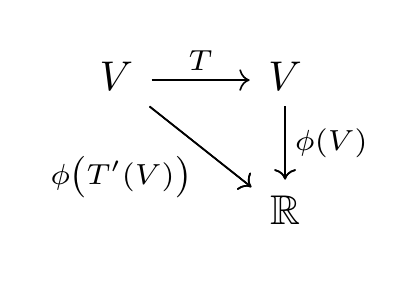
\begin{tikzpicture}[baseline = (a).base]
    \node[scale = 1.5] (a) at (0, 0){
        \begin{tikzcd}
            V \arrow[rd] \arrow[r, "T"] \arrow[rd, "\phi \left( T'(V) \right)", swap]
            & V \arrow[d] \arrow[d, "\phi(V)"] \\
            & \R
        \end{tikzcd}};
\end{tikzpicture} $$
This has more significant meaning in the context of an inner product space: the adjoint is the result of taking taking a linear mapping which operates on vectors from the inner product space and constructing a symmetric mapping which operates on dual vectors to the inner product space; the mapping is "symmetric" precisely because it's designed to commute with the linear mapping with respect to the inner product of the inner product space. However, an alternate perspective here is to view the inner product not as a defining characteristic of either $ V $ or $ W $ but rather as a way of specifying an isomorphism between each respective vector space and its dual space; the adjoint, then, and by extension (as we'll later show) the transpose, as a way of obtaining a symmetric "inverse" mapping of a mapping from $ V $ to $ W $ to a mapping from $ W^* $ to $ V^* $, in a way that commutes through this isomorphism. We can visualize the adjoint as "running the linear transform backwards"; indeed, one particular concrete case makes this intuition very clear, is that if we consider the adjacency matrix of a Markov chain (i.e. the matrix specifying transition probabilities), then its adjoint is the adjacency matrix for the Markov chain obtained by reversing all the edges of the original Markov chain, i.e. "running the transform backwards".
\nn
Let's solidify the intuition that, like the transpose, the adjoint is a kind of "dual inverse". In fact, in our discussion on the tranpose above, we touched on the same intuition that the transpose is a kind of "dual inverse" itself; here we'll further buttress this intuition and use it to elucidate the perspective that the adjoint is merely a reinterpretation of the transpose. Given any inner product space $ V $, we know that there's a natural (and canonical) isomorphism between $ V $ and its dual, $ V^* $, given by
    $$ \phi: V \rightarrow V^* \sti \forall v, w \in V: \phi(v)(w) = \langle v, w \rangle $$
In fact, as an aside, this definition of $ \phi $ makes it abundantly clear (once it's proven that $ \phi $ is actually linear and hence an isomorphism, though this follows easily from the axioms of an inner product) precisely why the inner product yields a natural isomorphism between a space and its dual. Anyway, given inner product spaces $ V $ and $ W $, this means there are corresponding isomorphisms $ \phi_V: V \rightarrow V^* $ and $ \phi_W: W \rightarrow W^* $ and hence, for linear transform $ T: V \rightarrow W $, we can interpret the map $ T^\intercal: W^* \rightarrow V^* $ as a map from $ W $ to $ V $, if we just use the isomorphisms as a looking glass first. More formally, we can consider the mapping
    $$ (\phi_V)^{-1}(T^\intercal)(\phi_W): W \rightarrow V $$
That is, we consider $ (\phi_V)^{-1} \circ T^\intercal \circ \phi_W: W \rightarrow V $. All we're doing here is reinterpreting $ T^\intercal $, initially defined as a mapping between $ W^* $ to $ V^* $, as a mapping from $ W $ to $ V $ by using the dual isomorphisms as looking glasses. If we unpack definitions, we'll find that the mapping 

TODO

\end{document}
